\chapter{File}
\section{目的}
熟悉linux中与文件操作相关的\textcolor{red}{系统调用}和\textcolor{red}{标准I/O库}。
\section{目标}
编写两个程序,分别使用系统调用和标准I/O库实现文件的拷贝。
\section{实验过程}
\subsection{准备知识}
\subsubsection{用户程序、库函数、系统调用与内核之间的关系}
用户程序、库函数、系统调用与内核之间的关系如Figure \ref{relation}所示。
\begin{figure}
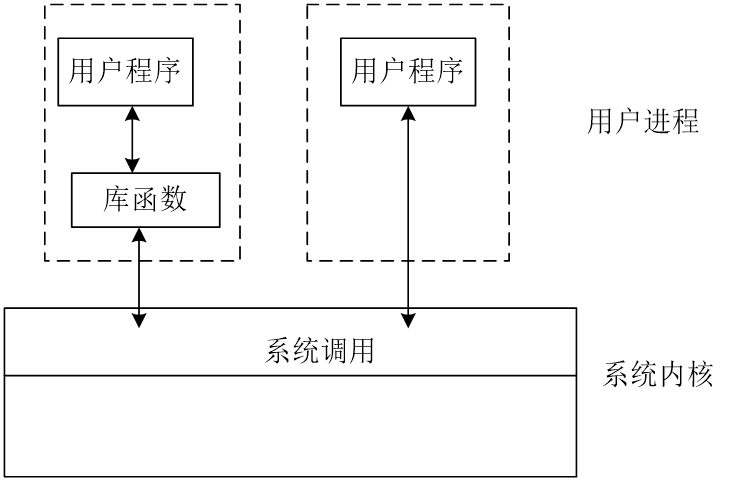
\includegraphics{601.png}
\caption{用户程序、库函数、系统调用与内核之间的关系}
\label{relation}
\end{figure}
\subsubsection{相关的系统调用}
\textbf{open}
\begin{lstlisting}
OPEN(2)                     BSD System Calls Manual 

NAME
     open, openat -- open or create a file for reading or writing

SYNOPSIS
     #include <fcntl.h>

     int
     open(const char *path, int oflag, ...);

     The flags specified for the oflag argument are formed by or'ing 
     the following values:

           O_RDONLY        open for reading only
           O_WRONLY        open for writing only
           O_RDWR          open for reading and writing
           O_NONBLOCK      do not block on open or for data 
                                          to become available
           O_APPEND        append on each write
           O_CREAT         create file if it does not exist
           O_TRUNC         truncate size to 0
           O_EXCL          error if O_CREAT and the file exists

\end{lstlisting}
\textbf{read}
\begin{lstlisting}
READ(2)                     BSD System Calls Manual 

NAME
     pread, read, readv -- read input

LIBRARY
     Standard C Library (libc, -lc)

SYNOPSIS
     #include <sys/types.h>
     #include <sys/uio.h>
     #include <unistd.h>

     ssize_t
     read(int fildes, void *buf, size_t nbyte);
\end{lstlisting}

\textbf{write}
\begin{lstlisting}
WRITE(2)                    BSD System Calls Manual

NAME
     pwrite, write, writev -- write output

LIBRARY
     Standard C Library (libc, -lc)

SYNOPSIS
     #include <unistd.h>



     ssize_t
     write(int fildes, const void *buf, size_t nbyte);

\end{lstlisting}
\textbf{close}
\begin{lstlisting}
CLOSE(2)                    BSD System Calls Manual 

NAME
     close -- delete a descriptor

SYNOPSIS
     #include <unistd.h>

     int
     close(int fildes);

\end{lstlisting}
\subsubsection{相关的库函数}
\textbf{fopen}
\begin{lstlisting}
FOPEN(3)                 BSD Library Functions Manual  

NAME
     fopen, fdopen, freopen, fmemopen -- stream open functions

LIBRARY
     Standard C Library (libc, -lc)

SYNOPSIS
     #include <stdio.h>

     FILE *
     fopen(const char * restrict path, const char * restrict mode);

The argument mode points to a string beginning with 
one of the following letters:

     ``r''   Open for reading.  The stream is positioned at
             the beginning of the file.  Fail if the file does not exist.

     ``w''   Open for writing.  The stream is positioned at 
             the beginning of the file.  Create the file if it does not exist.

     ``a''   Open for writing.  The stream is positioned at 
             the end of the file.  Subsequent writes to the file 
             will always end up at the then current end of file, 
             irrespective of any intervening fseek(3) or similar.  
             Create the file if it does not exist.

     An optional ``+'' following ``r'', ``w'', or ``a'' opens the file 
     for both reading and writing.
\end{lstlisting}
\textbf{fread、fwrite}
\begin{lstlisting}
FREAD(3)                 BSD Library Functions Manual 

NAME
     fread, fwrite -- binary stream input/output

LIBRARY
     Standard C Library (libc, -lc)

SYNOPSIS
     #include <stdio.h>

     size_t
     fread(void *restrict ptr, size_t size, size_t nitems, 
               FILE *restrict stream);

     size_t
     fwrite(const void *restrict ptr, size_t size, size_t nitems, 
               FILE *restrict stream);

DESCRIPTION
     The function fread() reads nitems objects, each size bytes long,
     from the stream pointed to by stream, storing them at the location
     given by ptr.

     The function fwrite() writes nitems objects, each size bytes long, 
     to the stream pointed to by stream, obtaining them from the location
     given by ptr.


\end{lstlisting}
\textbf{fclose}
\begin{lstlisting}
FCLOSE(3)                BSD Library Functions Manual  

NAME
     fclose, fcloseall -- close a stream

LIBRARY
     Standard C Library (libc, -lc)

SYNOPSIS
     #include <stdio.h>

     int
     fclose(FILE *stream);
\end{lstlisting}
\textbf{fgetc}
\begin{lstlisting}
GETC(3)                  BSD Library Functions Manual

NAME
     fgetc, getc, getc_unlocked, getchar, getchar_unlocked, getw 
       -- get next character or word from input stream

LIBRARY
     Standard C Library (libc, -lc)

SYNOPSIS
     #include <stdio.h>

     int
     fgetc(FILE *stream);

     int
     getc(FILE *stream);

     int
     getc_unlocked(FILE *stream);

     int
     getchar(void);

     int
     getchar_unlocked(void);

     int
     getw(FILE *stream);

DESCRIPTION
     The fgetc() function obtains the next input character (if present) from
          the stream pointed at by stream, or the next character 
          pushed back on the stream via ungetc(3).

     The getc() function acts essentially identically to fgetc(), 
         but is a macro that expands in-line.

     The getchar() function is equivalent to getc(stdin).
\end{lstlisting}
\textbf{fputc}
\begin{lstlisting}
PUTC(3)                  BSD Library Functions Manual 

NAME
     fputc, putc, putc_unlocked, putchar, putchar_unlocked, putw
      -- output a character or word to a stream

LIBRARY
     Standard C Library (libc, -lc)

SYNOPSIS
     #include <stdio.h>

     int
     fputc(int c, FILE *stream);

     int
     putc(int c, FILE *stream);

     int
     putc_unlocked(int c, FILE *stream);

     int
     putchar(int c);

     int
     putchar_unlocked(int c);

     int
     putw(int w, FILE *stream);

DESCRIPTION
     The fputc() function writes the character c 
       (converted to an ``unsigned char'') to the output stream
        pointed to by stream.

     The putc() macro acts essentially identically to fputc(), 
     but is a macro that expands in-line.  It may evaluate stream 
     more than once, so arguments given to putc() should not be
      expressions with potential side effects.

     The putchar() function is identical to putc() with an output 
        stream of stdout.
\end{lstlisting}
\subsection{使用系统调用实现文件拷贝}
使用系统调用逐个字符地拷贝文件,代码如Figure \ref{syscall}所示。
\begin{figure}
\begin{lstlisting}
#include <unistd.h>
#include <sys/stat.h>
#include <fcntl.h>
#include <stdlib.h>

int main(){
	char c;
	int in,out;
	
	in = open("simple_read.c",O_RDONLY);
	out = open("copy_example",O_WRONLY|O_CREAT,S_IRWXU);
	while(read(in,&c,1) ==1 ){
		write(out,&c,1);
		write(1,&c,1);
	}
	close(in);
	close(out);
	exit(0);
}

\end{lstlisting}
\caption{系统调用逐个字符拷贝}
\label{syscall}
\end{figure}
\subsection{使用标准I/O库实现文件拷贝}
\subsubsection{使用fread和fwrite函数实现}
使用fread和fwrite函数实现文件的拷贝,代码如Figure \ref{frdfwt}所示,\textcolor{red}{注意本程序有bug,请尝试发现并改正\footnote{参考fseek和ftell函数}}。
\begin{figure}
\begin{lstlisting}
#include <stdio.h>
#include <stdlib.h>
//fread fwrite have problems,
//the final part cannot be 
//written to the file.
int main(){
	int c;
	FILE *in, *out;
	char s[20];

	in = fopen("simple_read.c","r");
	out = fopen("io_copy","w+");
	c = fread(s,10,1,in);
	
	while(c>0){
		printf("%s",s);
		fwrite(s,10,c,out);
		c = fread(s,10,1,in);
		
	}
	fclose(in);
	fclose(out);
	exit(0);
}

\end{lstlisting}
\caption{使用fread和fwrite函数拷贝文件}
\label{frdfwt}
\end{figure}
\subsubsection{使用getc和putc函数实现}
使用getc和putc函数实现文件拷贝的代码如Figure \ref{getputc}所示。
\begin{figure}
\begin{lstlisting}
#include <stdio.h>
#include <stdlib.h>

int main(){
	int c;
	FILE *in;
	FILE *out;

	in=fopen("simple_read.c","r");
	out=fopen("io_copy_getcputc","w");
	while((c=fgetc(in))!=EOF){
		fputc(c,out);
	}
	fclose(in);
	fclose(out);
	exit(0);
}
\end{lstlisting}
\caption{使用getc和putc函数拷贝文件}
\label{getputc}
\end{figure}